\section{Introduction}
\label{sec:introduction}
Inpainting is an image processing technique used to infer the value of unknown pixels using the information apparent in the original image. One application for this method is image restoration where single pixels or larger scratches are missing, e.g. due to defective image acquisition or the age-driven deterioration of video footage. Another very common application is the removal of certain parts of an image, like watermarks or user-selected objects in the image. Figure \ref{fig:apps} shows examples for input images that can be treated by inpainting methods. Throughout this paper we assume that it is known beforehand which pixels have to be reconstructed. The extraction of defective regions in the image is not discussed here.

\begin{figure*}[t]
	\centering
	\begin{subfigure}{.5\columnwidth}
	   \centering
	   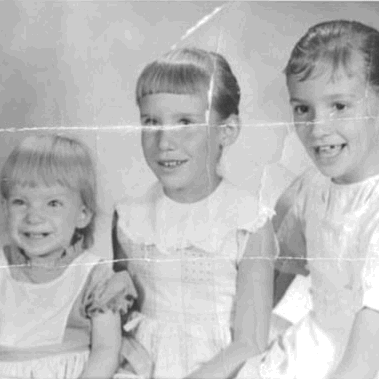
\includegraphics[width=.9\columnwidth]{graphics/3children_original_cropped.png}%
	      \caption{Image restoration
	      \label{fig:apps:image_restoration}
	   }
	\end{subfigure}\hfill%
	\begin{subfigure}{.5\columnwidth}
	   \centering
	   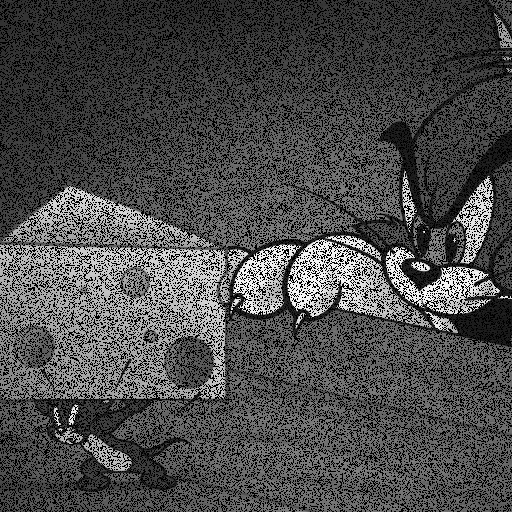
\includegraphics[width=.9\columnwidth]{graphics/TomAndJerry_512x512_pepper_in.png}%
	      \caption{Noise removal
	      \label{fig:apps:noise_removal}
	   }
	\end{subfigure}\hfill%
	\begin{subfigure}{.5\columnwidth}
	   \centering
	   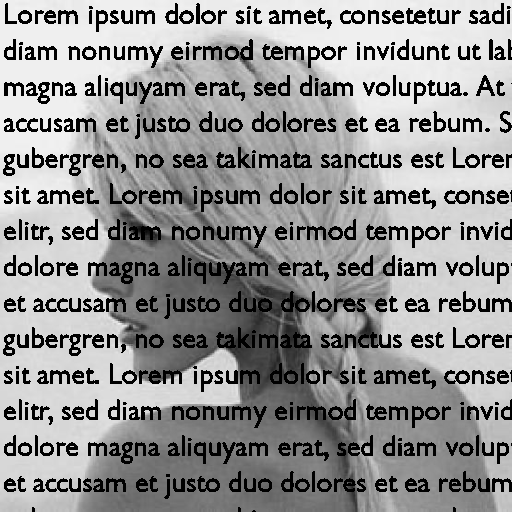
\includegraphics[width=.9\columnwidth]{graphics/claudia_512x512_mask_in.png}%
      	   \caption{Removal of watermarks
	      \label{fig:apps:watermarks}
	   }
	\end{subfigure}\hfill%
	\begin{subfigure}{.5\columnwidth}
	   \centering
	   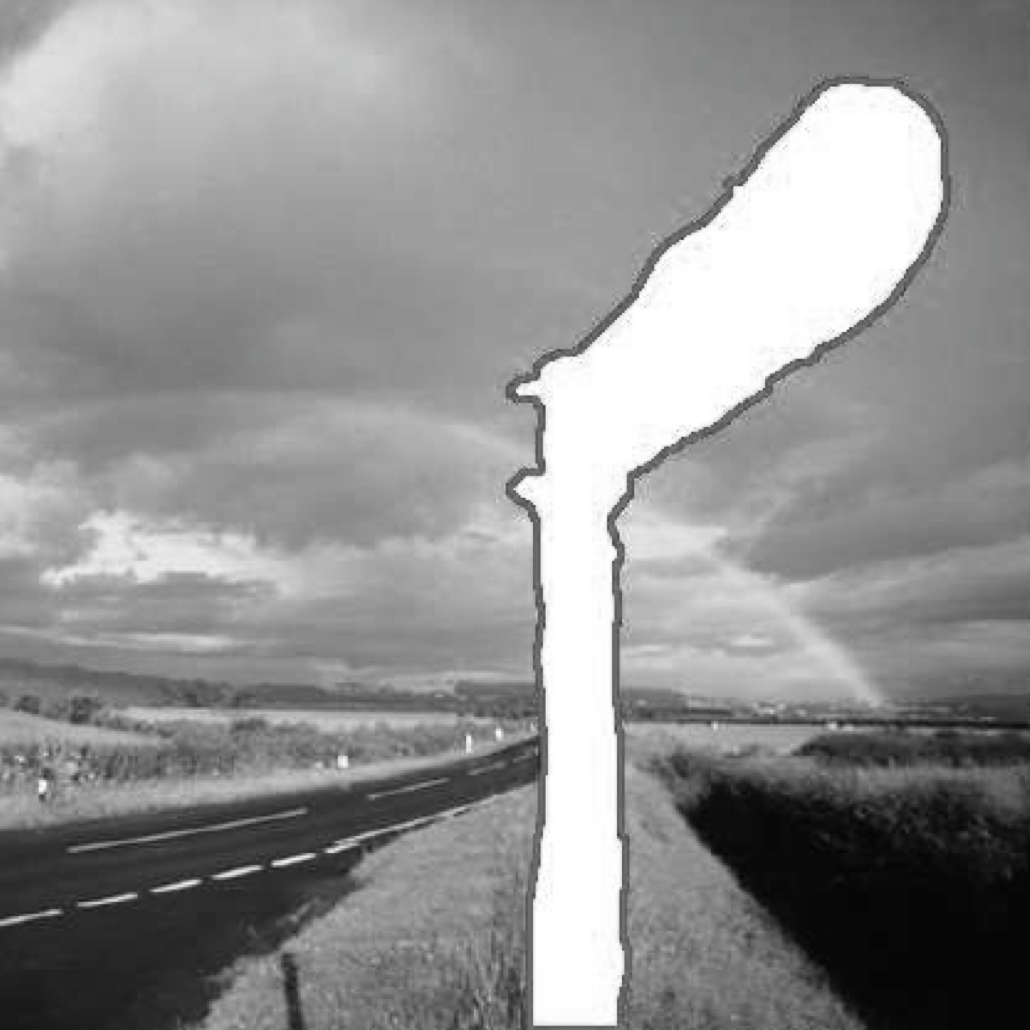
\includegraphics[width=.9\columnwidth]{graphics/object_removal_gray.png}%
      	   \caption{Object removal
	      \label{fig:apps:watermarks}
	   }
	\end{subfigure}\hfill%
	\caption{Sample applications for inpainting. [TODO: REF OF IMAGE SOURCES]
	   \label{fig:apps}
	}
\end{figure*}

\mypar{Existing work}
There exist many different techniques for inpainting, sometimes very specific to a certain application. For example noise reduction or recovering has been treated by various approaches using filter theory, Bayesian framework [TODO REFS]. Others [TODO REF] apply texture-synthesis approaches where the objective is to remove (potentially large) objects from an image by mimicking the surrounding region of the to-be-removed objected. Very popular in the image processing community is the exemplar-based method described by Criminisi et al., [REF CRIMINISI], an onion-peel approach where local gradients steer the fill-in procedure, which helps to preserve edges in the c. The correct reconstruction of the occluded region is of lesser importance in this approach and it impresses with a good overall visual perception.

\mypar{Our approach}
The method presented here is based on sparse coding of image patches. This technique can be compared with an interpolation scheme that takes into account . The results achieved with this method a

The novelty of our patch-based method consists of the combination of the following components:
\begin{itemize}
   \item Intelligent use of neighboring patches to support the sparse encoding of a patch.
   \item Learning a dictionary 
   \item Redundant reconstruction of missing pixels by overlapping patches and 
\end{itemize}

\mypar{Structure of the text} In section \ref{sec:methods} some background information about the proposed methods is presented. Section \ref{sec:results} presents our implementation which is then compared in the subsequent section \ref{discussion}. 